
\documentclass[12pt, a4paper]{report}
\usepackage[a4paper, total={6in, 8in}]{geometry}
\usepackage{hyperref}
%\usepackage{fourier-otf}
\usepackage[utf8]{inputenc}
\usepackage{graphicx}
\usepackage{algorithm}
\usepackage{algpseudocode}
\usepackage{float}
\usepackage{lipsum}
\usepackage{scrextend}
\usepackage{longtable}
\usepackage{biblatex}
\addbibresource{bibliography.bib}
\usepackage{listings}
\usepackage{amsmath}
\usepackage{amsfonts}
\usepackage{acro}
%\usepackage[square,sort,comma,numbers]{natbib}
\newtheorem{theorem}{Theorem}[section]
\usepackage{color}
\usepackage{makeidx}
\usepackage{titlepic}
%\usepackage{acronym}
\definecolor{mygreen}{rgb}{0,0.6,0}
\definecolor{mygray}{rgb}{0.5,0.5,0.5}
\definecolor{mymauve}{rgb}{0.58,0,0.82}
\newtheorem{remark}{Remark}
\lstset{ %
	backgroundcolor=\color{white},   % choose the background color
	basicstyle=\footnotesize,        % size of fonts used for the code
	breaklines=true,                 % automatic line breaking only at whitespace
	captionpos=b,                    % sets the caption-position to bottom
	commentstyle=\color{mygreen},    % comment style
	escapeinside={\%*}{*)},          % if you want to add LaTeX within your code
	keywordstyle=\color{blue},       % keyword style
	stringstyle=\color{mymauve},     % string literal style
}
\usepackage{hyperref}
\hypersetup{
	colorlinks   = true,    % Colours links instead of ugly boxes
	urlcolor     = black,    % Colour for external hyperlinks
	linkcolor    = black,    % Colour of internal links
	citecolor    = black      % Colour of citations
}
%\title{First chapter}

%\author{F.Bernardi}

%\protect\\ 

\newcommand{\myName}{Fabrizio Bernardi}
\newcommand{\myTitle}{Data analysis and modeling of calcium activity in   mice somatostatin interneurons}
\newcommand{\myDegree}{Programme: \protect\\ \textit{Mathematical Engineering} \\
	Academic years: 2021-2022}
\newcommand{\myCycle}{XXXI cycle}
\newcommand{\myDepartment}{Department of Mathematics}
\newcommand{\myUni}{Politecnico di Milano}
\newcommand{\myYear}{2022}
\newcommand{\myTime}{01 Jan \myYear}

\pdfbookmark{Cover}{cover}





\begin{document}



\chapter{Modeling calcium patterns}

In this final chapter, the mathematical tools discussed in Chapter 5 are put in practice, through a model which attempts to unify the given data of calcium peaks in neurons, with the electrophysiological process of action potentials propagation.\\
Indeed, the \textbf{Cable-Calcium} model considers a pair of neurons in which simultaneous calcium peaks have been recorded, and use such data to simulate, via cable model \ref{balance pde}, the propagation of an action potential from one cell to another. The goal is, given a calcium peak in the first neuron, to obtain a truthful estimation of the peak recorded in the second.\\ 
In the first part of the chapter, we discuss the connection between the intracellular calcium concentration and the corresponding action potential, in order to being able to use the cable model to simulate the propagation of the impulse from the first neuron to the second one. Once the link between calcium and action potential have been estimated, and the parameters of the cable model appropriately tuned, the cable simulation can start. This will lead to a predicted value of action potential at the end of the axon, giving rise to a corresponding value of calcium, to be compared with the acquired data. In the final part of the chapter, the model will be considered considering the different ways to model the conduction current, discussed in the previous chapter, comparing the results and commenting the performance of the model in the different cases.




\section{The Cable-Calcium model}

\begin{figure}[H]
	\begin{center}
		
		\includegraphics[scale=0.65]{cable_ca.png} 
	\end{center} 
	\caption{\textit{Schematic representation of the cable-calcium model.}}
	\label{cabel_ca}
\end{figure}

Let us consider a neuronal pair in which, from the recorded data of calcium activity, we have been able to identify two peaks of calcium occurred in a short time window (for the present case, chosen up to $0.5$ $s$). The main goal of the 
\textbf{Cable-Calcium} model is to being able to predict the amplitude of the peak in the second neuron, referred to as neuron B, given the peak occurred in the first neuron, referred to as neuron A, up to half second before.\\
From a biological point of view, we know that the presence of calcium peaks usually reflects the formation of action potentials in a cell, which then propogates through the axon to another cell. We discussed in Section \ref{section cable} how to mathematically model this process via Cable equation. The Cable-Calcium model, schematized in Figure \ref{cabel_ca}, consists in the following parts:

\begin{enumerate}
	
	\item Estimate the relation which connects the amplitude of a calcium peak (in terms of $\frac{\Delta F}{F})$ with the amplitude of the corresponding action potential. Use such relation to compute the action potential corresponding to the calcium peak recorded in neuron A \label{step1}
	
	\item The computed action potential will constitute a boundary condition at the beginning of the axon connecting A to B, for a cable model which simulate its propagation 
	
	\item The FE solution of the cable model, considered at the end of the axon, corresponds to the action potential occurred in neuron B. Using the inverse of the relationship estimated in step \ref{step1}, such value will identify a calcium value at neuron B \label{step3}
	
	\item In order to evaluate the goodness of the Cable-calcium model, the value of calcium in neuron B, obtained in step \ref{step3},  has to be compared with the actual value recorded from calcium imaging, in the same neuron.
	
\end{enumerate}


Mathematically, the cable model can be expressed in terms of calcium data as it follows:

\begin{equation}
	\begin{cases} 
	\frac{\partial \psi_m(x,t)}{\partial t} + \frac{1}{2 \pi a }\frac{\partial I_{in}(x,t)}{\partial x} + J_{cond}(x,t) = 0 & \text{in} \hspace{0.07 cm} (0,L) \times (0,T) \\ 
	I_{in}(x,t) = -\frac{\pi a^2}{\rho_{ax}}\frac{\partial \psi_m(x,t)}{\partial x} & \text{in} \hspace{0.07 cm} (0,L) \times (0,T) \\
	\psi_m(0,t) = \phi^{-1}([Ca_A^{2+}](t)) & \text{in} \hspace{0.07 cm} \left\{ x = 0\right\} \times (0,T) \\
	\psi_m(L,t) = \phi^{-1}([Ca_B^{2+}](t)) & \text{in} \hspace{0.07 cm} \left\{ x = L\right\} \times (0,T) \\
	\psi_m(x,0)=0  & \text{in} \hspace{0.07 cm}  (0,L) \times \left\{ t = 0\right\}
	\end{cases} \label{cable with ca}
\end{equation}	

where the boundary conditions at the beginning and at the end of the axon (i.e. in correspondence of neuron A and neuron B) are retrieved using the  function $\phi^{-1}$, which takes a  calcium peak  and gives out an action potential. The estimation of such function is discussed in the next Section.

\begin{remark}\label{remark cc}
	Eq. (\ref{cable with ca}) expresses a \textbf{dissipative} model: in the setting discussed so far, the action potential propagating along the axon can only diminuish its amplitude in space and time, because of the dissipation caused by the equivalent circuit assumed locally in every point $\textbf{x} \in [0,L]$. This means that the cable model considers the neuronal pair as isolated, so that the only process taken under consideration is the propagation of the potential from neuron A to neuron B. In reality, clearly this is not the general case: the neurons are present in a \textbf{network} and the formation of an action potential (or alternatively of a calcium peak) is the result of the interaction of more units. Moreover, it is also legit to assume that external contributions are added to the dissipative one in the transmission of the impulse, such as interaction with astrocytes or new stimuli captured by dendrites. For these reasons, observing the data, it is possible to find calcium peaks in neuron B which are higher than the ones in neuron A, meaning that the observed peak is the result of processes more complex than the simpler ones explained by the cable model. Finally, it is also worth to notice that observing simultaneous peaks does not necessarely means that the two neurons are actually biologically linked, since they could have both  been triggered, closely in time, by external neurons not present in the ROI  of the miniscope.
\end{remark}


As consequence of Remark \ref{remark cc}, the data considered in the model have been restricted to the neuronal pairs in which it could be clearly identified a \textit{pattern} of calcium firing (when neuron A shows a peak, neuron B does it as well), in which the same order is mantained (neuron A shows a peak always before neuron B), and the dissipative model can be justified (the peak in neuron B is lower than the one in neuron A). In this way, we may assume that the pair is well isolated, and fit to be considered for our model.

\section{The Ca-AP relation}


\begin{figure}[H]
	\begin{minipage}{\linewidth}
		\centering
		\begin{minipage}{0.45\linewidth}
			\begin{figure}[H]
				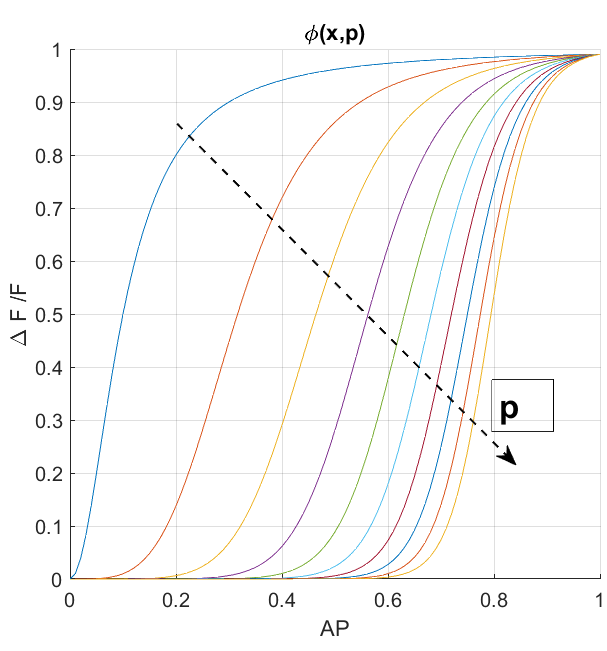
\includegraphics[width=\linewidth]{phi.png}
				
			\end{figure}
		\end{minipage}
		\hspace{0.05\linewidth}
		\begin{minipage}{0.45\linewidth}
			\begin{figure}[H]
				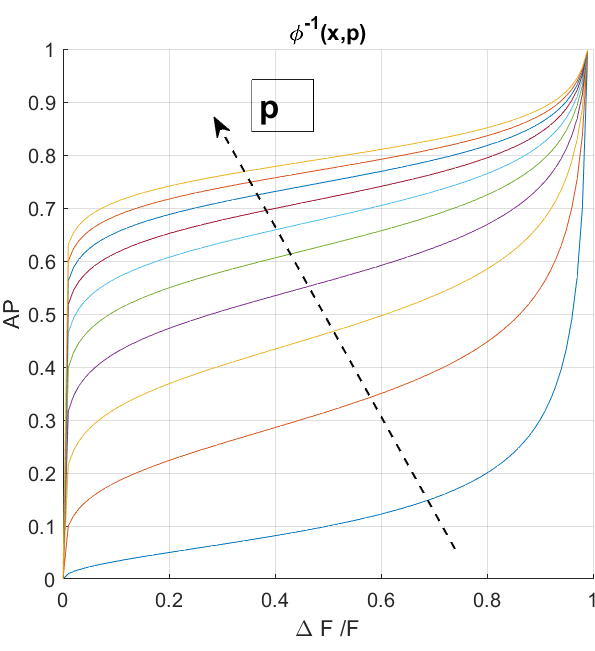
\includegraphics[width=\linewidth]{phi_inv.png}
				
			\end{figure}
		\end{minipage}
		
	\end{minipage}
	\caption{\textit{Plot of $\phi = \phi (x,p)$ for different values of $p \in [2,20]$.}}
	\label{phi}
\end{figure}

Finding a relation between calcium and action potential is a very difficult task. From a biological point of view, although we know that the presence of a calcium peak is usually related to the formation of an action potential, the microscopic mechanisms which regulate this connection are still largely unknown. This is mostly due to the fact that the dynamic of the intracellular calcium is the result of complex mechanisms inside the cell, given by a balance of fluxes between the cytoplasm and organules like \textit{mitochondria}, but mostly between cytoplasm and \textbf{calcium buffers} present in the cell \cite{43}. Although we know that these processes are triggered by action potentials, mathematical descriptions of this relation, especially for specific cases of neurons like the one studied in this work, are missing or insufficients.\\
Therefore, the best approach to estimate the relationship between the two quantity would probably be a data-driven relation estimated from simultaneous measurements of the two quantities, for example estimating the relationship via an Artifical Neural Network. Unfortunately, the literature doesn't seem to present many information about simultaneous recording of calcium and action potential for our specific needs, namely SOM+ interneurons in the ACC. For this reason, we went for a different approach: the estimation of the function connecting the two world as a parameter-dependent function, built from an educated guess on its shape.\\
In order to simplify the task, we limited ourselves to consider only the \textit{amplitude} of the peaks, associating to every calcium peak a single value given by its maximum, and relating to it a corresponding value for the peak of action potential. Such value will be the boundary condition at $x=0$ in Eq. \ref{cable with ca}, given as constant impulse in a certain time window (here set at $250$ $ms$ in accordance with experimental evidence).\\

Next, data have been appropriately normalized in the interval $[0,1]$, via \textit{min-max normalization} discussed in Section \ref{norm}. The maximum and minimum values for the signal have been directly computed for the calcium oscillations, while for the action potential it has been set

\begin{equation}
\psi_m ^{min}= -67 \hspace{0.2cm} mV \hspace{2cm}	\psi_m ^{max} = 20 \hspace{0.2cm} mV
\end{equation}
 
So that the non-activity state, assumed at the equilibrium potential $\psi_m = -67$ $mV$, is associated to the value $0$, and the maximum peak, which in practice usually approaches values of $20$ $mV$, is associated to the value $1$.\\
In this setting, the functions $ \phi : [0,1] \rightarrow [0,1] $, which takes a normalized value of action potential as input, and returns a normalized value of calcium as output, and $ \phi^{-1} : [0,1] \rightarrow [0,1] $, which takes a normalized value of calcium as input, and returns a normalized value of action potential as output, have been built on the following assumptions:

\begin{enumerate}
	\item $\phi$ is  an \textit{increasing} function (so that higher peaks of action potential correspond to higher peaks of calcium) \label{hp1}
	
	\item $\phi (0) = 0 $, $\phi (1) = 1 $, corresponding to an equilibrium state at $\psi_m = \psi_m ^{min}$ and to the maximum peak at  $\psi_m = \psi_m ^{max}$
	
	\item $\phi$ has a \textit{sigmoidal-like} shape \label{sigm}
\end{enumerate}

Assumption \ref{sigm} relies on the biological property of  action potentials for which they tend to assume an ON/OFF behaviour, based on a certain treshold value.\\
A function  $\phi$ which gets in well accordance with hypothesis 1.-3. is

\begin{equation}
	\phi(x,p) = \frac{x^p}{k + x^p}
\end{equation}

Where it has been set $k=0.01$ (in order to get close to hypothesis \ref{hp1}) and $p \in \mathbb{N}$ is a parameter to be optimally tuned. Its inverse is

\begin{equation}
\phi^{-1}(x,p) = \sqrt[p]{\frac{kx}{1-x}}
\end{equation}

These two functions, plotted over different values of $p$, are showed in Figure \ref{phi}.


\section{Setting the cable parameters}

Once that the function connecting calcium and action potential has been established, many parameters used in the cable model have to be tuned. The chosen values are the result of experimental evidences or previous results in the literature. The main choices are displayed in Table \ref{param}.\\
Some parameters come directly from the experimental calcium data, and have to be set appropriately in every call to the FE library:

\begin{itemize}
	\item The length of the axon $L$ is retrieved from the distance between the two considered neurons in the ROI
	
	\item The final time of the simulation $T$ is taken as $t_B - t_A$, being $t_A$ and $t_B$ the times in which the calcium peak happened in neurons A and B, respectively
	
\end{itemize}




As for the boundary conditions, the choice has been the following:

\begin{equation}
	\begin{cases}
	\psi_m(0,t) = \phi^{-1}([Ca_A^{2+}])(\psi_m^{max} - \psi_m^{min}) + \psi_m^{min} & \text{in} \hspace{0.07 cm} \left\{ x = 0\right\} \times (0,T) \\
	-I_{in}(L,t) +\frac{1}{R_{out}}\psi_m(L,t) =0 & \text{in} \hspace{0.07 cm} \left\{ x = L\right\} \times (0,T)
	\end{cases} \label{bc}
\end{equation}

The first of \ref{bc} expresses the already mentioned imposition that the action potential in neuron A is retrived from the recorded calcium peak thanks to the function $\phi^{-1}$. For the second choice, the \textit{Robin} boundary condition, discussed in Section \ref{section cable}, has been adopted with $R_{out} \rightarrow \infty$, so that the current at neuron B is null. This choice wants to reflect the \textit{inhibitory behaviour} of the neuronal population under observation (recalling that SOM+ interneurons are inhibitory GABA cells, as mentioned in Section \ref{first section}).

\begin{table}[H]
	\begin{center}
		\begin{tabular}{ |c|c|c|c| } 
			\hline
			\textbf{Parameter} & \textbf{Name} & \textbf{Chosen value} \\
			\hline
			$t_m$ & Membrane thickness & $10^{-9}$ $ m$ \\ 
			\hline
			$\rho_{ax}$ & Axon resistivity & $10$ $\Omega$ $ m$ \\
			\hline
			$K_{in}/K_{out}$ & Ion number densitiy (Potassium) & $140/5$ $m^{-3}$ \\
			\hline
			$Na_{in}/Na_{out}$ & Ion number density (Sodium) & $10/145$ $m^{-3}$ \\
			\hline
			$Cl_{in}/Cl_{out}$ & Ion number density (Chlorine) & $4/110$ $m^{-3}$ \\
			\hline
			$C_m$ & Membrane capacitance & $0.07$ $F$ \\
			\hline
			$g_m$ & Specific membrane conductance & Model dependent \\
			\hline
			$M_h$ & Number of FE element in space & $200$ \\
			\hline
			$N_T$ & Number of FE element in time & $200$ \\
			
			
			\hline
		\end{tabular}
		
	\end{center}
	\caption{\textit{Main parameters of the Cable-Calcium model}. \cite{47}} \label{param}
\end{table}

\section{Workflow of the Cable-Calcium model}


The Cable-calcium model follows three main steps:

\begin{enumerate}
	\item \textbf{Data preparation}. The data of the neuronal pairs are collected, keeping the record of time and peak amplitude for the calcium peak in one neuron, and of the distance between neurons characterizing the pairs. as already discussed, only data corresponding to well isolated pairs are considered
	
	\item \textbf{Training}. Part of the dataset (approximately $ 60 \%$) is used to train the model: for every value of the parameter $p$, ranging in an appropriate  interval, and for all the pairs considered, a  FE simulation is launched, imposing the boundary condition  $\psi_m(0,t) = \phi^{-1}([Ca^{2+}_A])$. The predicted value of AP at the end of the axon will produce the predicted calcium peak in neuron B as $\phi(\psi_h(L,T))$, being $\psi_h$ the FE solution. Such value will be compared to the recorded data of $[Ca^{2+}_B]$. Computing, for every $p$, the \textbf{mean squared error (MSE)} between calcium prediction and calcium recordings in neuron B, we are finally able to determine the value of $p$ which minimizes such error. The MSE between two sequences $\textbf{x} = \{x_i\}_{i=1}^N$ and $\textbf{y} = \{y_i\}_{i=1}^N$ is computed as
	
	\begin{equation}
	MSE(\textbf{x},\textbf{y}) = \frac{1}{N}\sum_{i=1}^{N}(x_i-y_i)^2
	\end{equation}
	
	\item \textbf{Test}. The optimal value of $p$ is used on the other part of the dataset, in order to evaluate the goodness of the model, as predictive tool, on new data
	
\end{enumerate}




The three steps of the model have been performed with the three different ways to model the conduction current, discussed in the previous chapter:  the \textbf{linear resistor model (LRM)}, the \textbf{Goldman-Hodgkin-Katz (GHK)} model and finally the \textbf{Hodgkin-Huxley (HH)} model. The dataset for the training consisted in $11$ recorded pairs, while the one for the testing in $8$. Such pairs have been selected in order to satisfy the hypotheses discussed in Remark \ref{remark cc}.

\section{Results of the Cable-Calcium model}


\begin{figure}[H]
	\begin{center}
		\hspace*{-1.6 cm}
		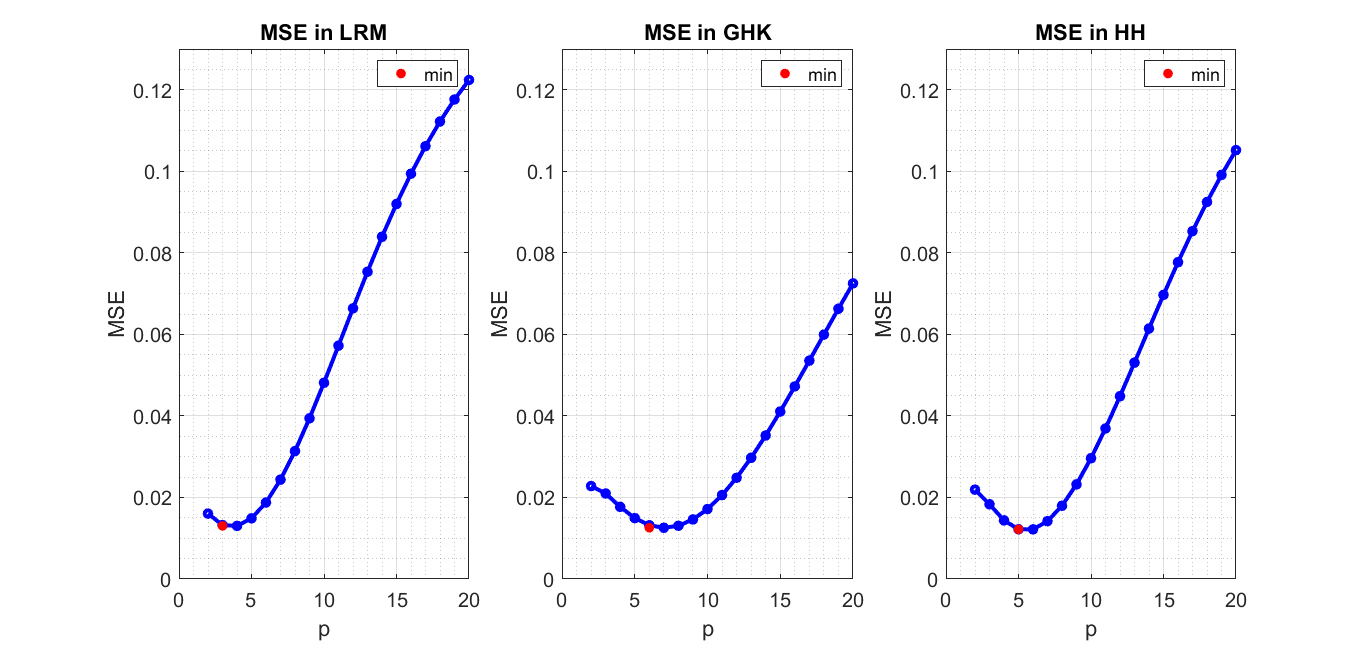
\includegraphics[scale=0.5]{MSE.png} 
	\end{center} 
	\caption{\textit{Mean squared error for the predictions on the training pairs, computed for different values of $p$. Left: in LRM model. Center: in GHK model. Right: in HH model. }}
	\label{mse}
\end{figure}

The training of the model in the three choices of LRM, GHK and HH produced the results showed in Figure \ref{mse}. In all the cases, ranging $p$ in the interval $[2,20]$ made it possible to identify a global minimum for the MSE. Every model resulted in a different optimal value of $p$ and produced a different error. Figure \ref{training_LRM}, considering as example the LRM case, shows that the choice of $p$ is fundamental in order to obtain significant predictions on the measured peaks in neuron B.\\ Confronting the predictions obtained in every model by the selection of the best value of $p$ (i.e. the value minimizing the MSE), it is immediately evident that, overall, the three models produce similar results  (Figure \ref{training}).
\begin{figure}[H]
	\begin{center}
		\hspace*{-1.5 cm}
		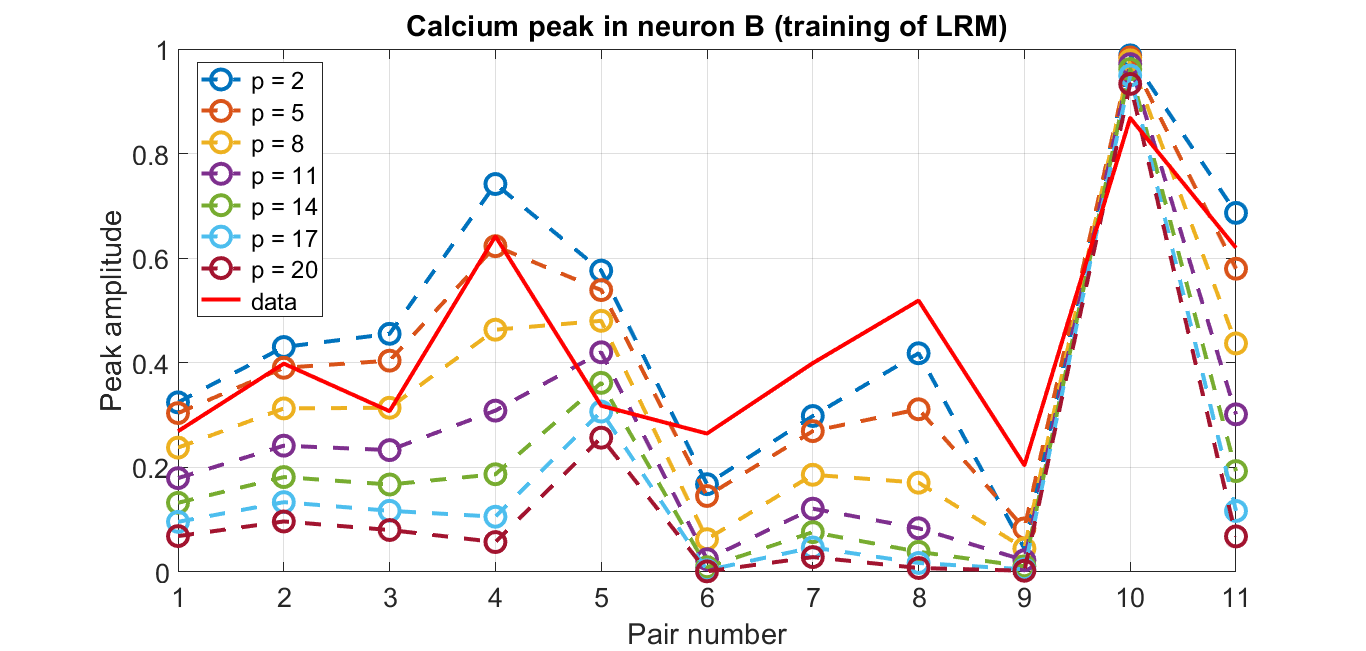
\includegraphics[scale=0.5]{training_LRM.png} 
	\end{center} 
	\caption{\textit{Predictions of calcium peaks in neuron B over the different neuronal pairs in the training dataset, using different values of $p$, for the LRM case.}}
	\label{training_LRM}
\end{figure}

\begin{figure}[H]
	\begin{center}
		\hspace*{-1.5 cm}
		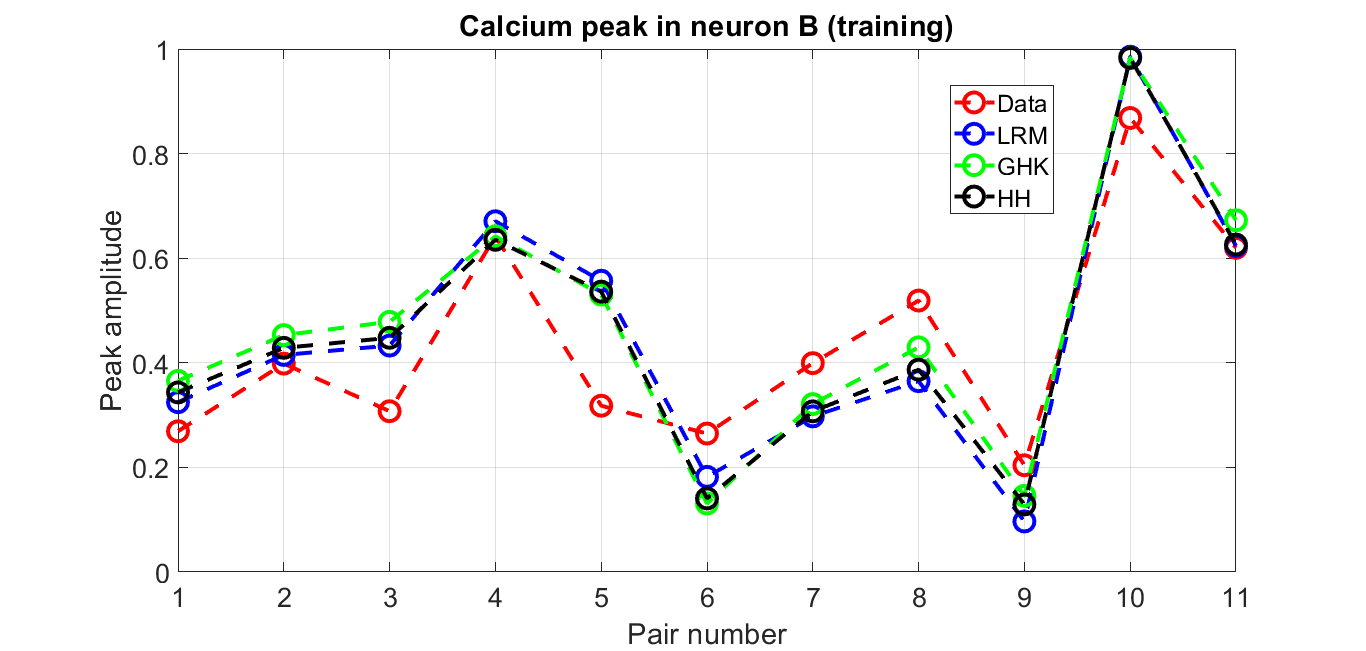
\includegraphics[scale=0.5]{training.png} 
	\end{center} 
	\caption{\textit{Predictions of calcium peaks in neuron B over the different neuronal pairs in the training dataset, for every different model. Every model corresponds to the choice of the value of $p$ which minimizes the MSE for all neuronal pairs.}}
	\label{training}
\end{figure}


Once the training process is completed, we can evaluate the performance of the model on the test data, using the value of $p$ which minimzes the MSE over the training data.\\
The results of the predictions in the different neuronal pairs are showed in Figure \ref{test}. We can observe that, as expected, the prediction is not as good as in the training case. Once again, the difference in the several choices of model is generally small, with the exception of some isolated pairs.\\
Table \ref{results} resumes all the principal results obtained in training and testing of the model.


\begin{table} [H]
	\centering
	\begin{tabular}{ |c|c|c|c| } 
		
		\hline
		\textbf{Model} & \textbf{LRM} & \textbf{GHK} & \textbf{HH} \\
		\hline
		\textbf{Best $p$ (training)}  & $p=3$ & $p=6$ & $p=5$ \\
		\hline
		\textbf{MSE at best $p$ (training)}  & $0.0130$ & $0.0126$ & $0.0122$  \\
		\hline
		\textbf{MSE at best $p$ (test)}  & $0.0203$ & $0.0182$ & $0.0179$  \\
		\hline
		
		
	\end{tabular} \caption{\textit{Main results of the Cable-Calcium model}.\label{results}}
\end{table}


	


\begin{figure}[H]
	\begin{center}
		\hspace*{-1.5 cm}
		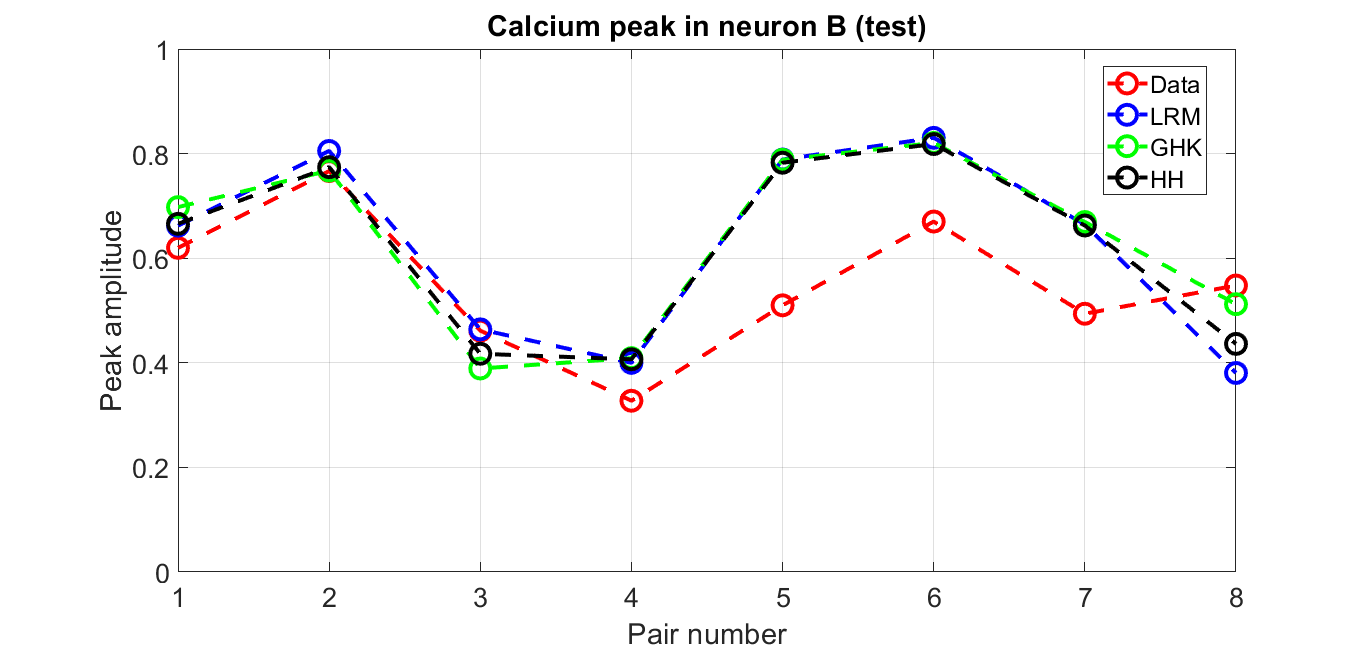
\includegraphics[scale=0.5]{test_model.png} 
	\end{center} 
	\caption{\textit{Predictions of calcium peaks in neuron B over the different neuronal pairs in the test dataset, for every different model. Every model corresponds to the choice of the value of $p$ which minimizes the MSE over the training data.}}
	\label{test}
\end{figure}

\section{Conclusions on the Cable-Calcium model}

Through the Cable-Calcium model, we attempted to predict the calcium peak triggered in one neuron, as consequence of the peak in another neuron. Analyzing the results in Table \ref{results}, one can notice several aspects.\\
Qualitatively, the three models perform in a similar way in predicting the calcium peaks, but small differences can be appreciated: for more complex nonlinearities assumed by the model, correspond smaller errors in the prediction (from the LRM to the HH case).\\
The similar behaviour of the prediction among the three model suggests the fact that the relevant contribution to the performance is actually given by the parameter optimization. Indeed, training all the three models using the same target data, it is likely that the differences on the overall results between them are flattened by the different choice of the optimal $p$, performed in each case, which allow to ultimately retrieve  similar results.\\
Clearly, this model constitutes a first attempt to model a very complex phenomenon, as the several hypotheses assumed to simplify it can testify. It follows that next works, based on it, could try to relax one by the one the simplifications of the model, making it always more realistic. In particular, we propose the following suggestions for future improvements:


\begin{itemize}
	\item The relationship $\phi$ could be improved, both in term of guess on its shape, and in terms of parameters. For example, one could think about letting vary also the parameter $k$
	
	\item The high differences in the prediction results obtained for different values of $p$, showed in Figure \ref{training_LRM}, suggest that this model could be improvable enlarging the interval considered for the parameter to vary. For example, one could think to let $p$ assume also decimal values. It is worth to notice, however, that this could be time-consuming, since for every value of $p$ and for every neuronal pair, a FE simulation is launched, consuming a considerable amount of time (especially in the Hodgkin-Huxley case). Similar considerations stand for considering larger training and testing datasets
	
	\item External effects of excitatory type could be included. In this case, one should clarify how to appropriately model them, performing a modification of the cable model itself
	
	\item Extensions to more neurons could be considered, with the ultimate goal to predict the calcium patterns in a \textit{network} of neurons, instead that in only one pair. This is clearly the most difficult step, since it is hard to corroborate experimentally (one should register in the ROI all the neurons involved in the network, a priori unknwon and/or not all capturable by a single minoscope lens)
	
\end{itemize}  



\end{document}